\section{محدودیت‌ها، تخمین‌ها و شرایط رضایتمندی}

\subsection{محدودیت‌ها}
\subsubsection{زمان شروع}
بسته با محتوای آموزشی و گذارندن دوره‌های آموزشی لازمه برای پروژه، هر قسمت زمان تا حدی متغیر دارد.
\subsubsection{سررسید‌ها}
پروژه در سال ۱۴۰۱ خورشیدی انجام می‌گیرد
\begin{itemize}
    \item تحویل پیشنهادنامه - ۱۶ اردیبهشت
    \item تحویل مستند تحلیل - ۶ خرداد
    \item تحویل مستند طراحی - ۲۷ خرداد
    \item ارائه‌ی نهایی محصول - ۲۸ مرداد
\end{itemize}
\subsubsection{بودجه‌ها}
با توجه به فشردگی برنامه‌ی دانشجویان، برنامه‌ی مشخص شده در بدبینانه‌ترین حالت ۱۲۶ روز طول خواهد کشید. بودجه نهایی معادل ۱۶۹/۳۴۴ میلیون تومان خواهد بود.
\begin{itemize}
    \item ۱۵ درصد به صورت پیشش پرداخت
    \item ۳۵ درصد پس از اتمام فاز سوم پیاده‌سازی
    \item ۵۰ درصد پس از اتمام پروژه
\end{itemize}
\subsubsection{تکنولوژی}
تصمیم تیم بر آن است که این پروژه بر بستر وب پیاده‌سازی شود. از جمله علل اصلی می‌توان به موارد زیر اشاره کرد
\begin{enumerate}
    \item با توجه به نیازمندی به یک رابط کاربری گیرا و مناسب طبیعتا نیازمند یک برنامه‌ی وب یا اپلیکیشن هستیم.
    \item جهت دسترسی از طریق تمامی وسایل هوشمند، برنامه‌ی وب گزینه‌ی مناسب و کم‌هزینه‌ای است.
    \item باتوجه به قرارگیری \lr{API}های مکالمه‌ی تصویری، احتمالا صفحه‌ی بزرگتر مناسب‌تر باشد و احتمالا تمایل رایانه‌ی رومیزی یا لپ‌تاپ بیشتر است.
    \item همه‌ی اعضای تیم آشنایی مختصری با بستر وب دارند.
\end{enumerate}

\subsection{برآورد‌ها}
\subsubsection{برآورد زمانی}
جدول زمانی پیش‌بینی شده‌ی پروژه به صورت زیر خواهد بود. همچنین نمودار گانت نیز پیوست شده است.
ضمنا با توجه به فشردگی برنامه‌ی دانشجویان پروژه در روزهای چهارشنبه، پنجشنبه و جمعه از ساعت ۳ تا ۷ بعدازظهر انجام خواهد گرفت. مشکلات عقب‌مانده نیز طی دیگر ساعات هفته مرتفع می‌شوند.

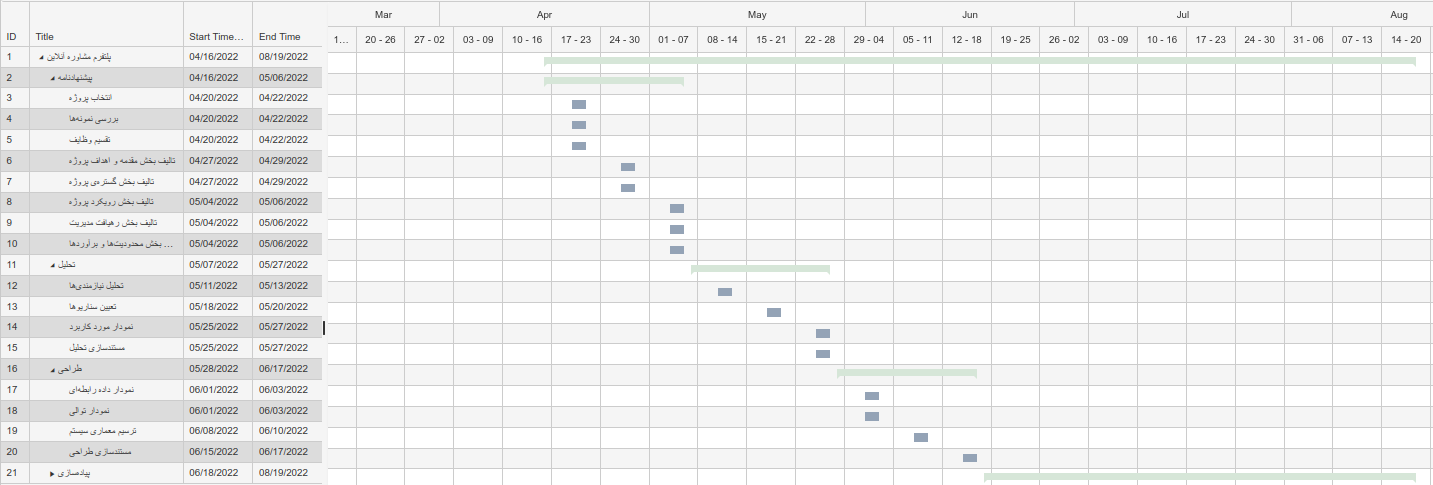
\includegraphics[width=1\textwidth]{Images/Gantt_1.png}
\newline
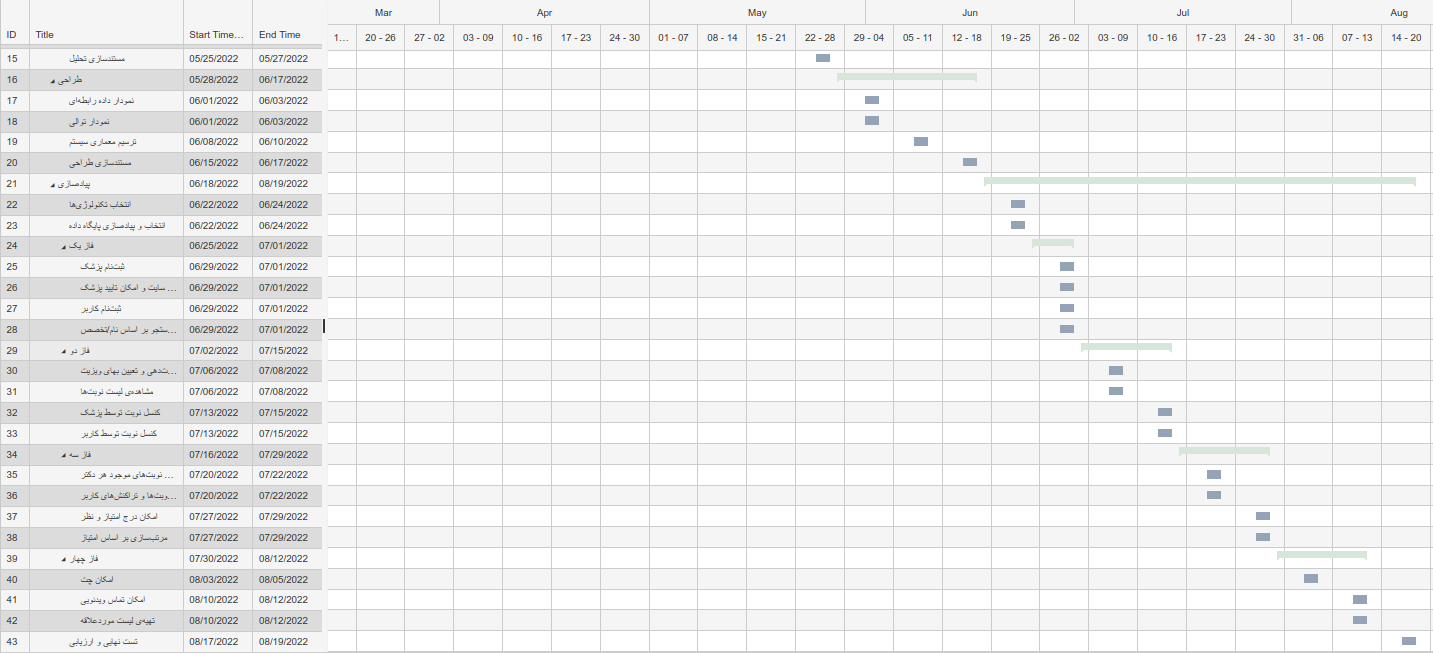
\includegraphics[width=1\textwidth]{Images/Gantt_2.png}

\subsubsection{برآورد مالی}
دستمزدها با توجه به شرایط مالی این حوزه و تجربه‌ی افراد به صورت زیر خواهد بود
\begin{itemize}
    \item یاشار ظروفچی - ساعتی ۲۸۰ هزار تومان معادل ۱۰ دلار
    \item فرزام زهدی‌نسب - ساعتی ۲۵۲ هزار تومان معادل ۹ دلار
    \item علی بالا‌پور - ساعتی ۲۵۲ هزار تومان معادل ۹ دلار
\end{itemize}

\subsubsection{برآورد هزینه‌ها}


\begin{table}
\centering
\resizebox{10cm}{!}{
\begin{tabular}{|c|c|c|}
\hline
هزینه  & نام بخش                & ID \\ \hline
6048\$   & سامانه مشاوره‌ی آنلاین & ۱  \\ \hline
1008\$ & پیشنهادنامه            & ۲  \\ \hline
1008\$ & تحلیل                  & ۱۱ \\ \hline
1008\$ & طراحی                  & ۱۶ \\ \hline
3024\$   & پیاده‌سازی             & ۲۱ \\ \hline
\end{tabular}%
}
\end{table}


\subsection{شرایط رضایتمندی}
\subsubsection{معیار‌های موفقیت}
در این قسمت، معیار‌هایی را مشخص می‌کنیم که تعیین کننده‌ی این هستند که پروژه با موفقیت به اتمام رسیده یا خیر. کنتر و نظرات بر این موارد در مراحل مختلف پروژه، به عهده‌ی مدیر پروژه است که می‌توان به موارد زیر اشاره کرد
\begin{enumerate}
    \item برخورداری از کیفیت مناسب
    \item اتمام پروژه در زمان مقرر
    \item اتمام پروژه با بودجه‌ی مشخص
\end{enumerate}
\subsubsection{پیش‌فرض‌ها}
تعدای از پیش‌فرض‌های پروژه در اینجا ذکر شده‌اند
\begin{itemize}
    \item کارجویان همگی دانشجوی دانشگاه صنعتی شریف هستند
    \item اطلاعات واردشده توسط کاربران معتبر هستند
    \item ادمین وبسایت به اطلاعات کاربران دسترسی خواهد داشت
    \item فعال بودن این سامانه از لحاظ حقوقی بلامانع است
\end{itemize}
\subsubsection{ریسک‌ها}
\begin{itemize}
    \item تغییر خواسته‌های کارفرما، که به تغییر برنامه‌ی زمانی یا ملی منجر خواهد شد
    \item کناره‌گیری یکی از اعضای تیم
    \item رونمایی از سامانه‌ی رقیب
\end{itemize}
